\documentclass[10pt]{article}
\usepackage[margin=3cm]{geometry}
\usepackage{amssymb}
\usepackage{verbatim}
\usepackage{graphicx}
\usepackage{amsmath}
\usepackage{capt-of}
\title{\bfseries\Huge Bram van den Akker}

\date{}
\begin{document}
\title{Cuda}
\author{Abe Wiersma, Bram van den Akker}
\date{\today}
\maketitle
\newpage

\section{Wave equation with cuda}
\textit{Because we're unable to complete part 1 of assignment 3 the results are only compared to assignment 1 and 2. }

In figure 1 you can clearly see that cuda performance is much higher that cpu multithreading when using large datasets. Where Pthreads and openMP need a lot of time to calculate the wave with an $i$ of $10^7$ cuda doesn't have much trouble getting fast results.


\begin{figure}[h]
  \centering
    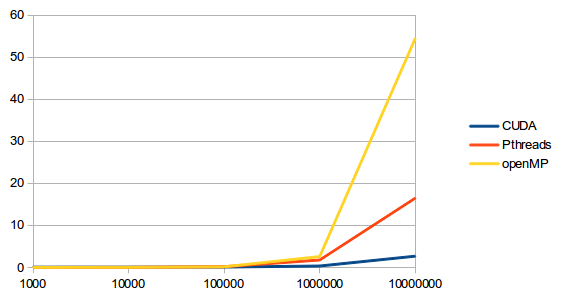
\includegraphics[width=\textwidth]{123compare.png}
  \caption{Cuda vs pthreads and openmp. Cuda block size is 512, pthreads and openmp both use 8 cores.}
\end{figure}
\break

\subsection{Blocksizes}
As you can see in the graph below a higher block size does not directly relate to a higher performance. When using block sizes larger than the amount of cores available the performance will go down (a GTX-480 has 448 cuda cores, this is why 512 is slower than 256 cores). Small blocksizes (i.e. 8, 16 and 32) will exceed the maximum amount of blocks when trying to run large datasets and fail. 
\begin{figure}[h]
  \centering
    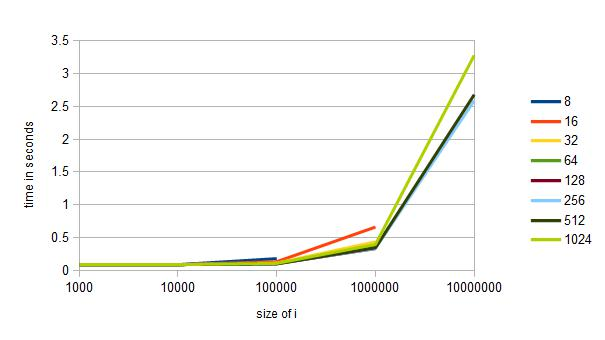
\includegraphics[width=\textwidth]{threadblocksizes-1000timesteps.jpg}
  \caption{Cuda scheduling with different block sizes.}
\end{figure}
\break

\subsection{Result comparison}
When using a small $i$ the results of the cuda implementation are really inaccurate, increasing the $i$ value will get much better results. This could be due to the use of floats instead of doubles. Float performance on cuda machines is much better although when dealing with small values lose a lot of precision. figure 4 through 8 show the cuda and pthreads results side by side. All results used $t_{max} = 1000$

\begin{figure}[h]
  \centering
    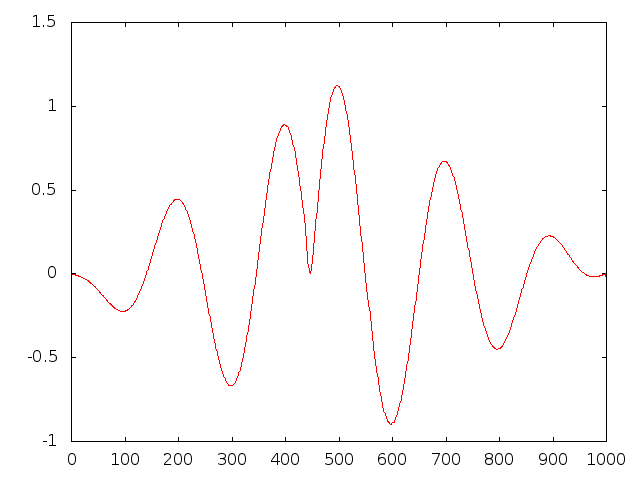
\includegraphics[width=\textwidth]{assign1_1000.png}
  \caption{Correct result of $i$ = 1000.}
\end{figure}
\break
\begin{figure}[h]
  \centering
    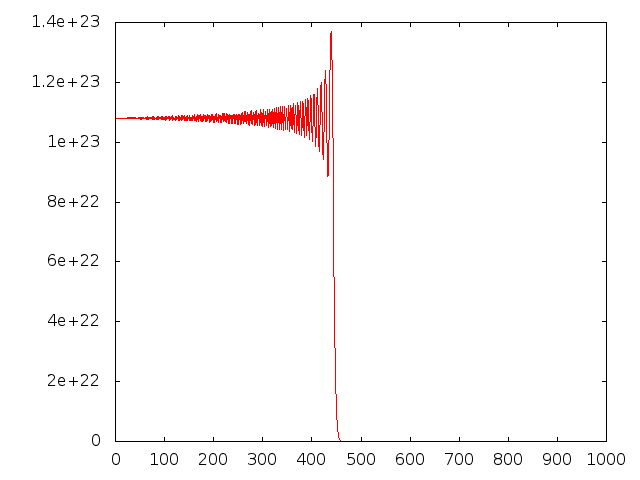
\includegraphics[width=\textwidth]{assign4_1000.png}
  \caption{Cuda result of $i$ = 1000.}
\end{figure}
\break

\begin{figure}[h]
  \centering
    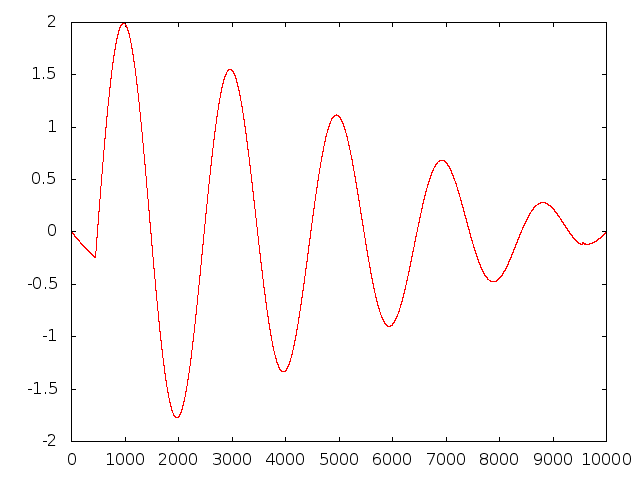
\includegraphics[width=\textwidth]{assign1_10000.png}
  \caption{Correct result of $i$ = 10000.}
\end{figure}
\break
\begin{figure}[h]
  \centering
    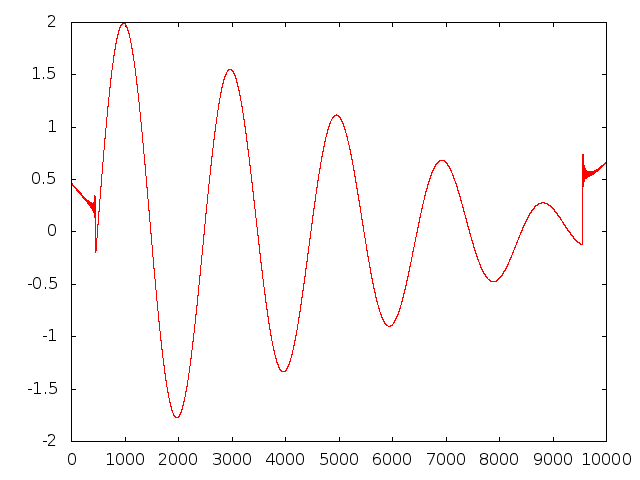
\includegraphics[width=\textwidth]{assign4_10000.png}
  \caption{Cuda result of $i$ = 01000.}
\end{figure}
\break

\begin{figure}[h]
  \centering
    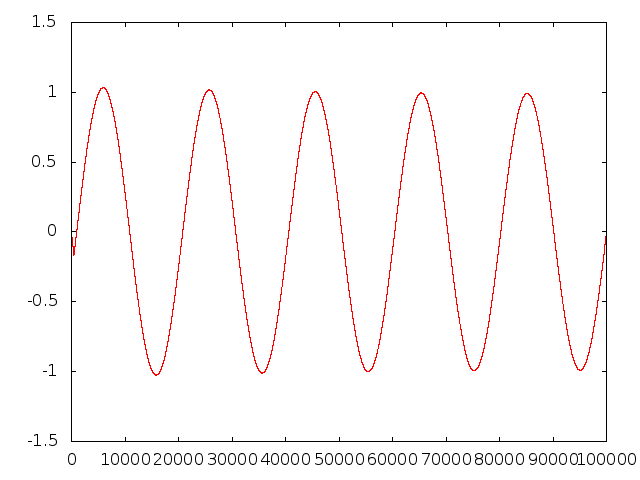
\includegraphics[width=\textwidth]{assign1_100000.png}
  \caption{Correct result of $i$ = 100000.}
\end{figure}
\break
\begin{figure}[h]
  \centering
    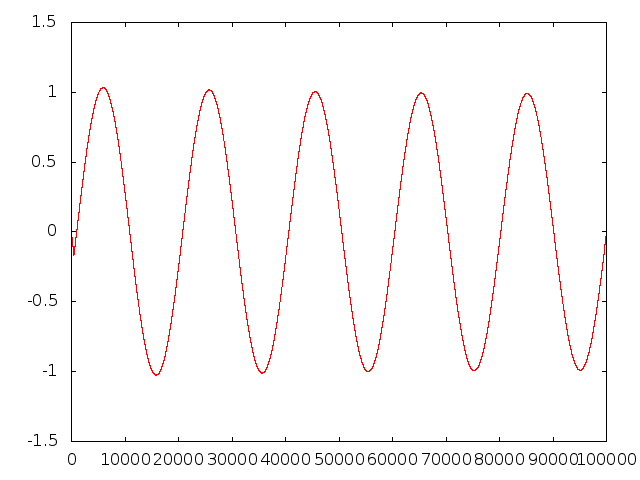
\includegraphics[width=\textwidth]{assign4_100000.png}
  \caption{Cuda result of $i$ = 100000.}
\end{figure}
\break


\section{Finding the max value}
When running both a cpu and cuda algorithm to find the maximum value of an array of floats one thing is really important: Array length. With a small amount of float values the CPU algorithm will perform better then the cuda algorithm. When the amount of float values is increased the cuda algorithm starts out performing the cpu algorithm. 
\\


\begin{tabular}{c | c | c}
N floats & cpu & cuda \\
10000 & 0.044096 $ms$ & 0.244032 $ms$ \\
1000000 & 4.19827 $ms$ & 1.60947 $ms$ \\
100000000 & 419.26 $ms$ & 117.667 $ms$\\
\end{tabular}
\\
The performance of the cpu algorithm vs the cuda algorithm. 

\end{document}